\subsection{Simulation }
Our simulation is based on two softwares: MATLAB(SimBiology Toolbox) and COPASI.

SimBiology Toolbox provides functions for modeling, simulating, and analyzing biochemical pathways by the powerful computing engine of MATLAB.

\begin{figure}[h]
	\centering
	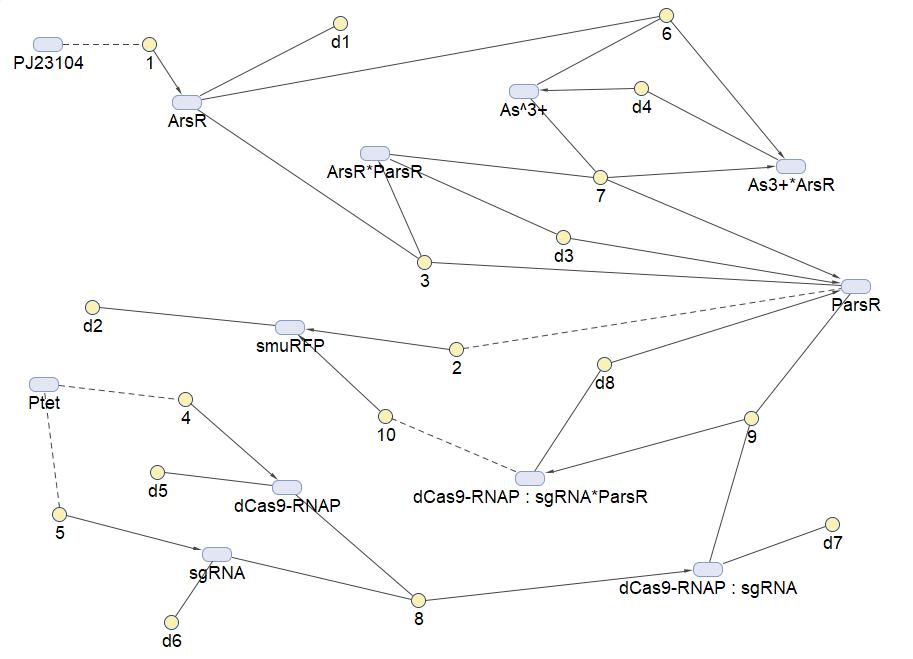
\includegraphics[width=10cm]{screenshot003}	
	\caption{Reaction map generated from the reaction sets above by SimBiology Toolbox}
\end{figure}



\begin{figure}[H]
	\centering
	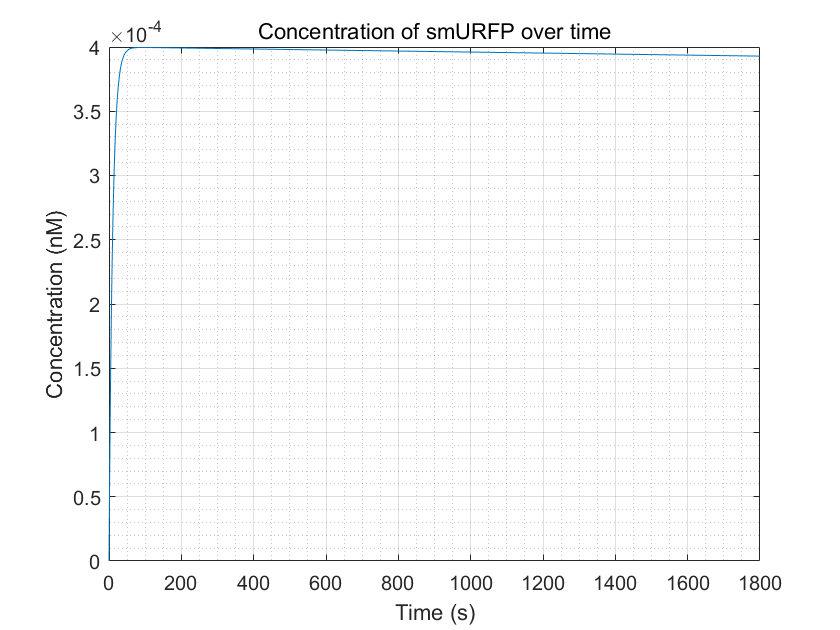
\includegraphics[width=10cm]{11}
	\caption{Simulation of smURFP production as a function of time by MATLAB}
\end{figure}

Through the figure, we can see that the smURFP can gradually increase and reach a steady state after a period in the presence of arsenic ions.

\subsection{Sensitivity }
A good biosystem should have certain stability towards fluctuations in parameters. A good model should reflect this, and hence a test for robustness can be essential to the model.

Robustness analysis can also pinpoint which reactions/parameters that are important for obtaining a specific biological behavior. A simple measure for sensitivity is to measure the relative change of a system feature due to a change in a parameter. As for our model, the feature can be the equilibrium concentration of the smURFP(C) for which the sensitivity (S) to a parameter k is:
\begin{equation}
	S=\frac{\frac{dC}{C}}{\frac{dk}{k}}=\frac{dC}{dk}\frac{k}{c}\approx \frac{\Delta C}{\Delta k}\frac{k}{c}
\end{equation}
\begin{figure}[H]
	\centering
	\begin{subfigure}{0.5\textwidth}
		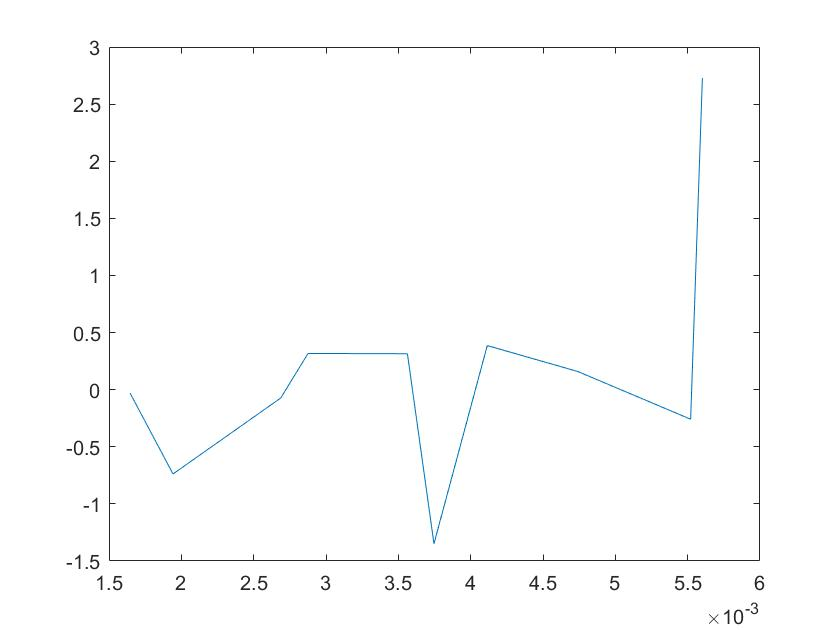
\includegraphics[height=4cm]{s1.jpg}
		\caption{sensitivity of k1}
	\end{subfigure}
	\begin{subfigure}{0.5\textwidth}
		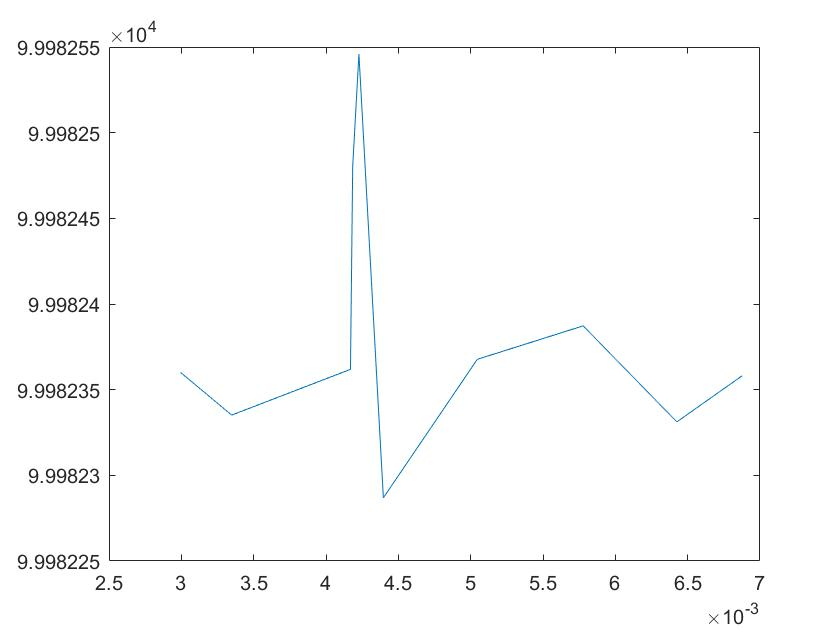
\includegraphics[height=4cm]{s2.jpg}
		\caption{sensitivity of k2}
	\end{subfigure}
	\begin{subfigure}{0.5\textwidth}
		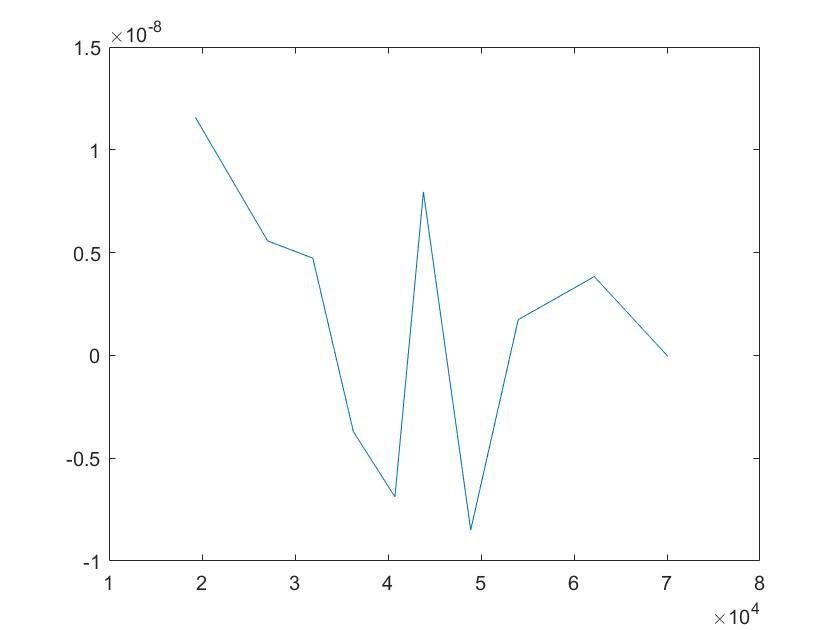
\includegraphics[height=4cm]{s3.jpg}
		\caption{sensitivity of k3}
	\end{subfigure}%
	\begin{subfigure}{0.5\textwidth}
		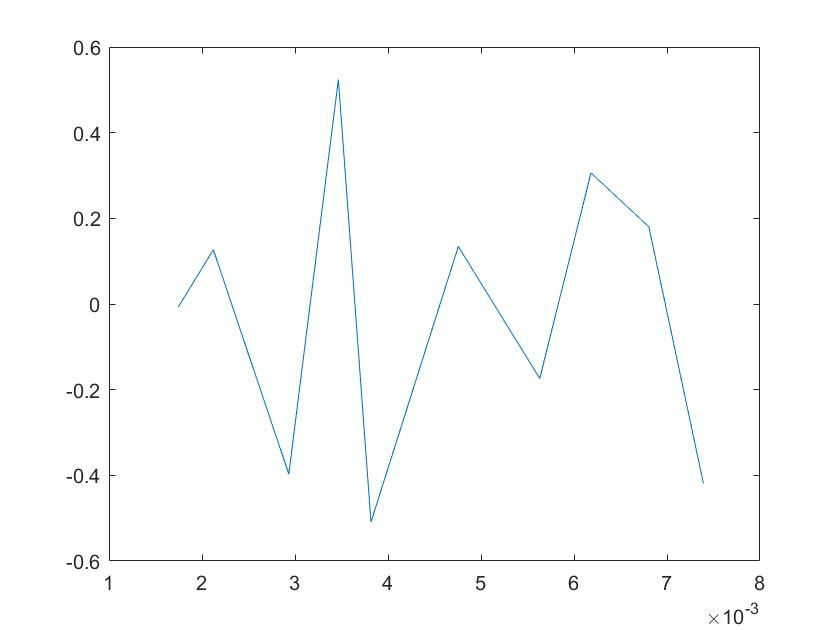
\includegraphics[height=4cm]{s4.jpg}
		\caption{sensitivity of k4}
	\end{subfigure}
	\begin{subfigure}{0.5\textwidth}
		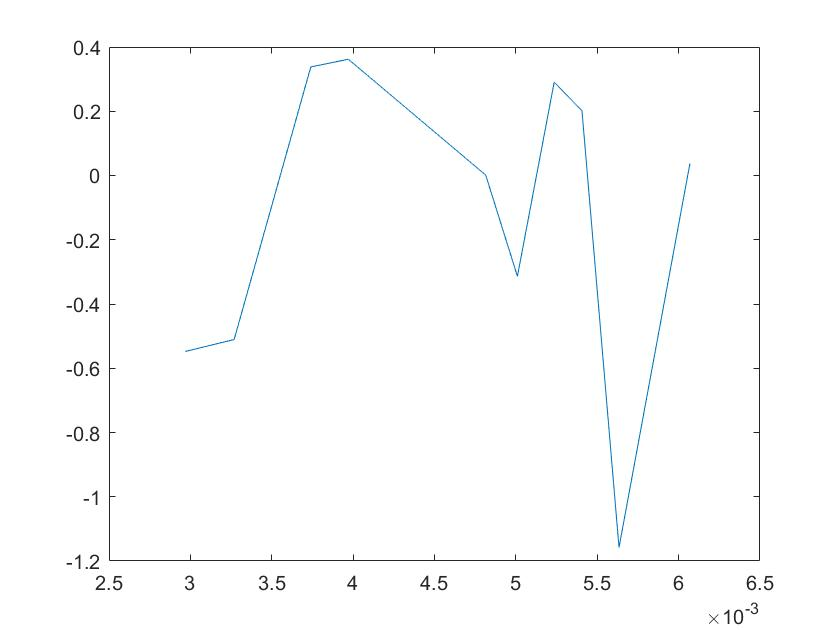
\includegraphics[height=4cm]{s5.jpg}
		\caption{sensitivity of k5}
	\end{subfigure}%
	\begin{subfigure}{0.5\textwidth}
		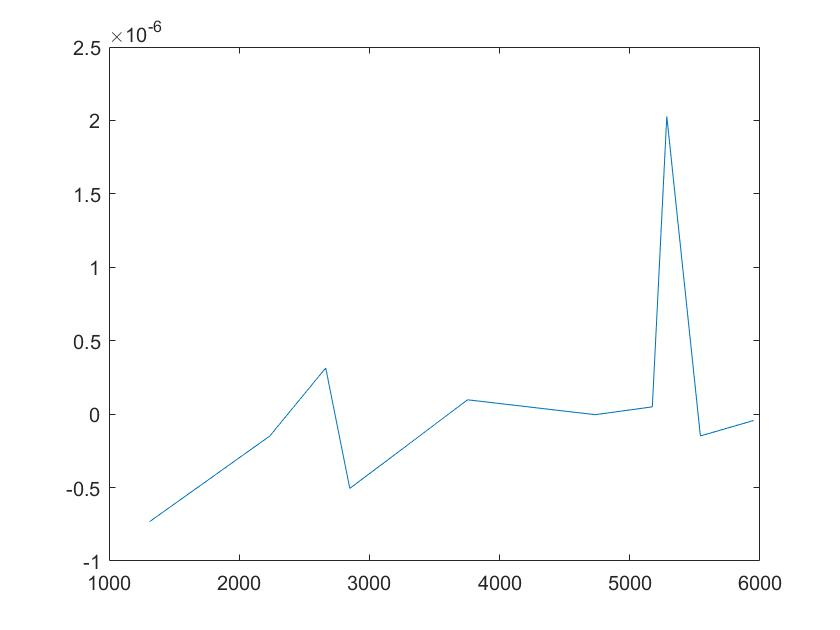
\includegraphics[height=4cm]{s6.jpg}
		\caption{sensitivity of k6}
	\end{subfigure}
	\begin{subfigure}{0.5\textwidth}
		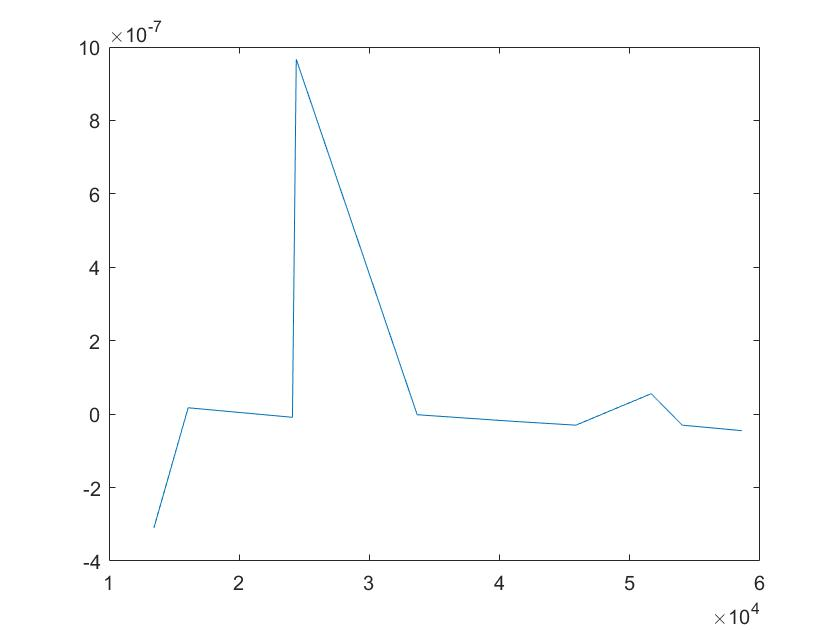
\includegraphics[height=4cm]{s7.jpg}
		\caption{sensitivity of k7}
	\end{subfigure}%
	\begin{subfigure}{0.5\textwidth}
		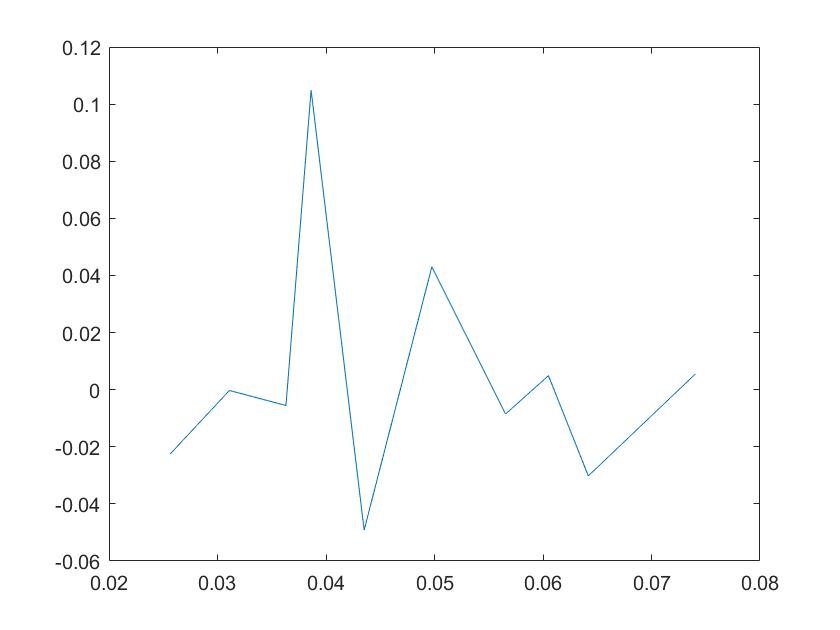
\includegraphics[height=4cm]{s8.jpg}
		\caption{sensitivity of k8}
	\end{subfigure}
	\begin{subfigure}{0.5\textwidth}
		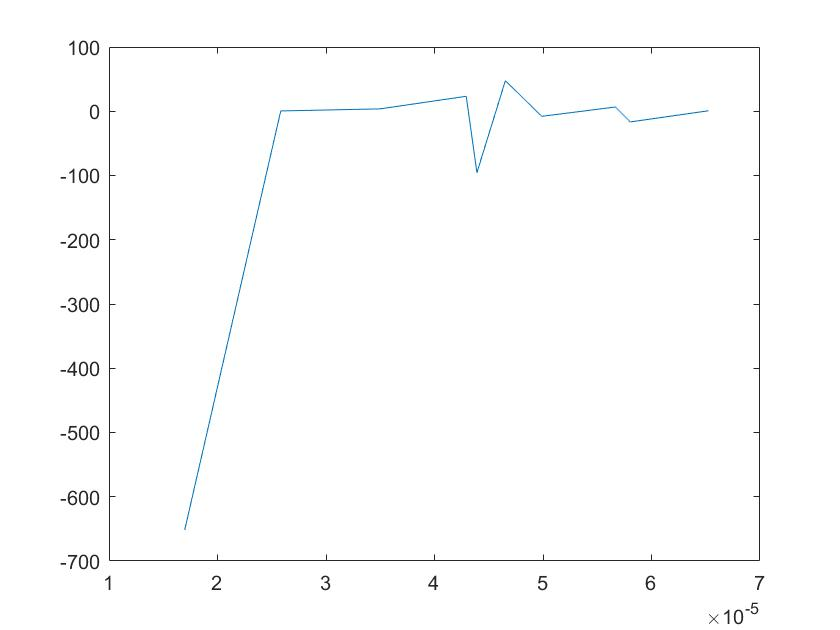
\includegraphics[height=4cm]{s9.jpg}
		\caption{sensitivity of k9}
	\end{subfigure}%
	\begin{subfigure}{0.5\textwidth}
		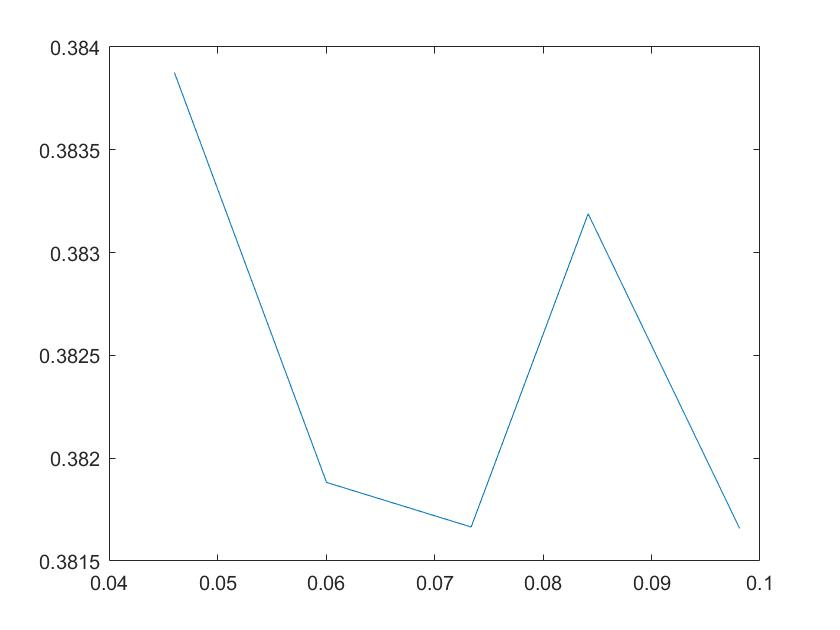
\includegraphics[height=4cm]{s10.jpg}
		\caption{sensitivity of k10}
	\end{subfigure}
	\caption{Sensitivity analysis of k1-k10}
\end{figure}

\begin{figure}[H]
	\begin{subfigure}{0.5\textwidth}
		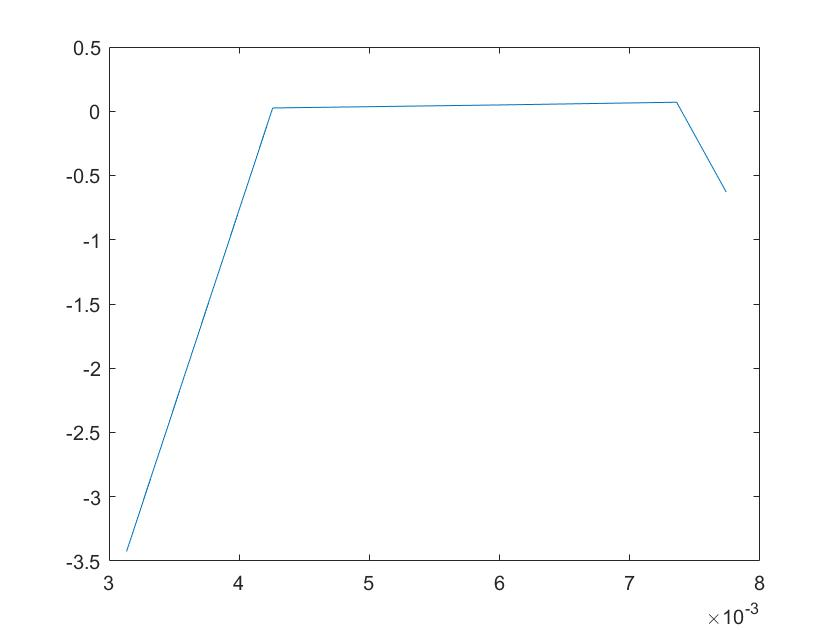
\includegraphics[height=4cm]{sd1.jpg}
		\caption{sensitivity of kd1}
	\end{subfigure}%
	\begin{subfigure}{0.5\textwidth}
		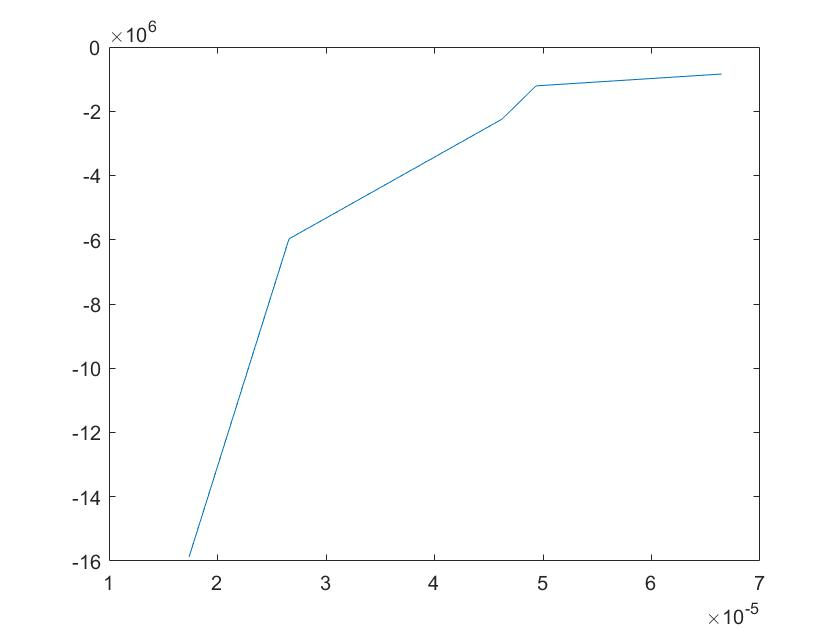
\includegraphics[height=4cm]{sd2.jpg}
		\caption{sensitivity of kd2}
	\end{subfigure}
	\begin{subfigure}{0.5\textwidth}
		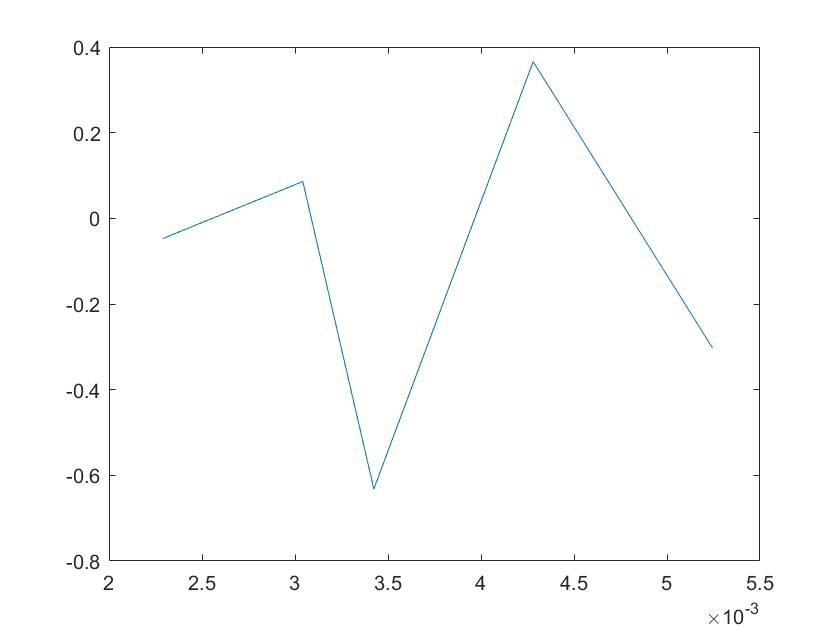
\includegraphics[height=4cm]{sd3.jpg}
		\caption{sensitivity of kd3}
	\end{subfigure}%
	\begin{subfigure}{0.5\textwidth}
		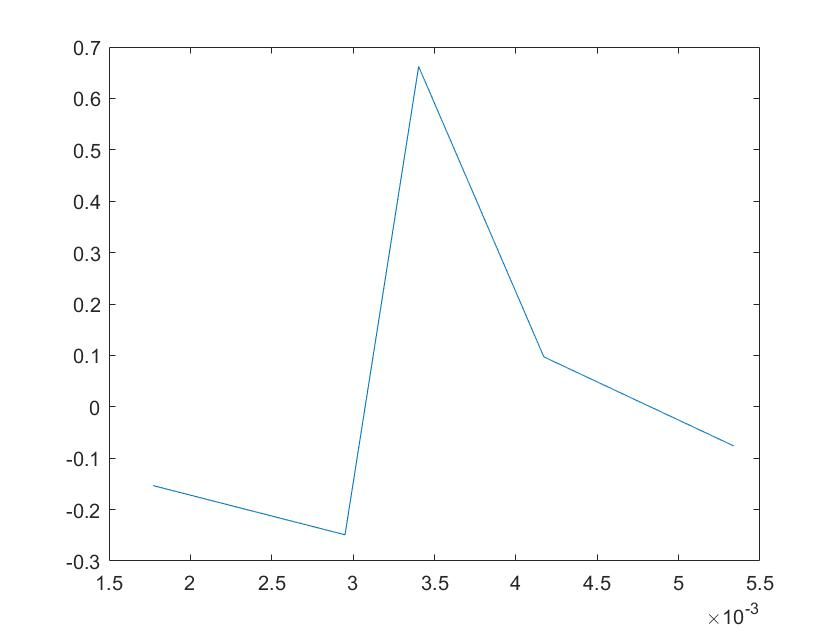
\includegraphics[height=4cm]{sd4.jpg}
		\caption{sensitivity of kd4}
	\end{subfigure}
	\begin{subfigure}{0.5\textwidth}
		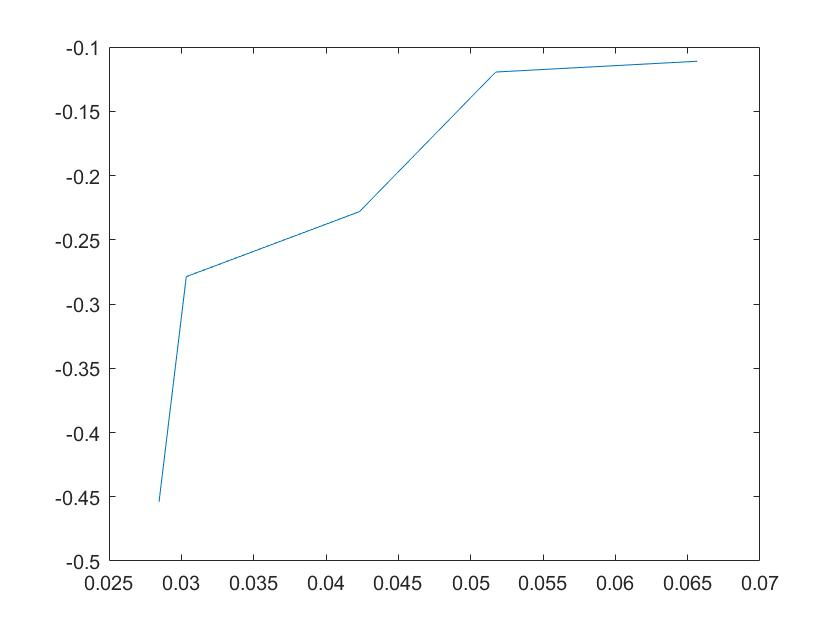
\includegraphics[height=4cm]{sd5.jpg}
		\caption{sensitivity of kd5}
	\end{subfigure}%
	\begin{subfigure}{0.5\textwidth}
		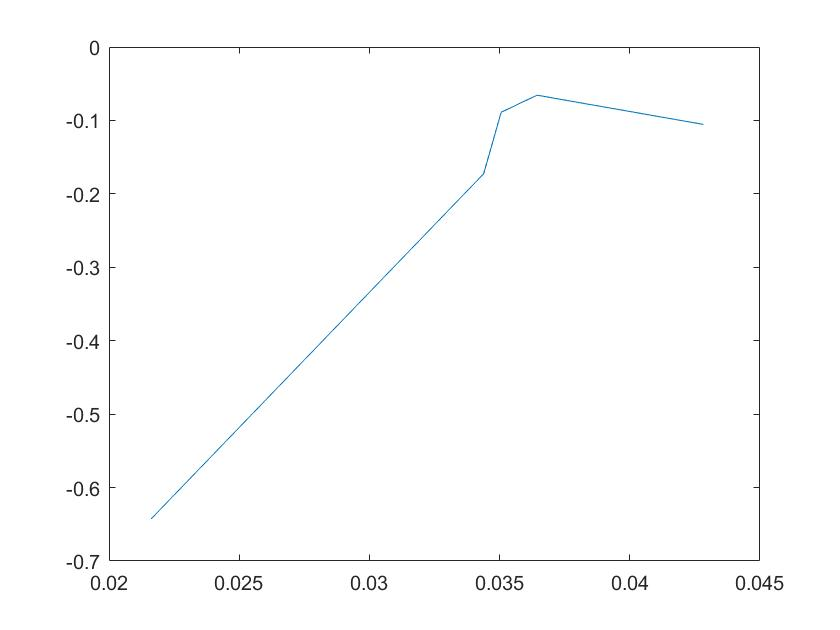
\includegraphics[height=4cm]{sd6.jpg}
		\caption{sensitivity of kd6}
	\end{subfigure}
	\begin{subfigure}{0.5\textwidth}
		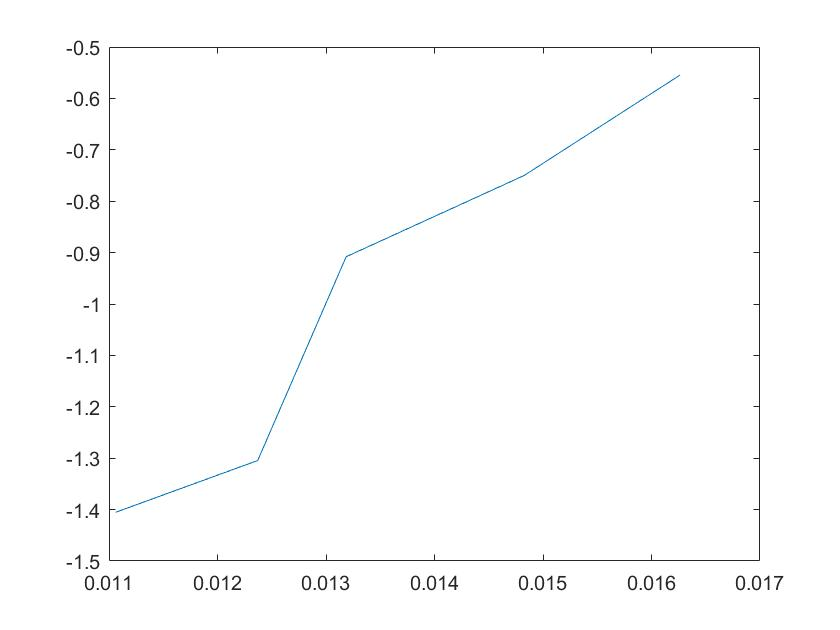
\includegraphics[height=4cm]{sd7.jpg}
		\caption{sensitivity of kd7}
	\end{subfigure}%
	\begin{subfigure}{0.5\textwidth}
		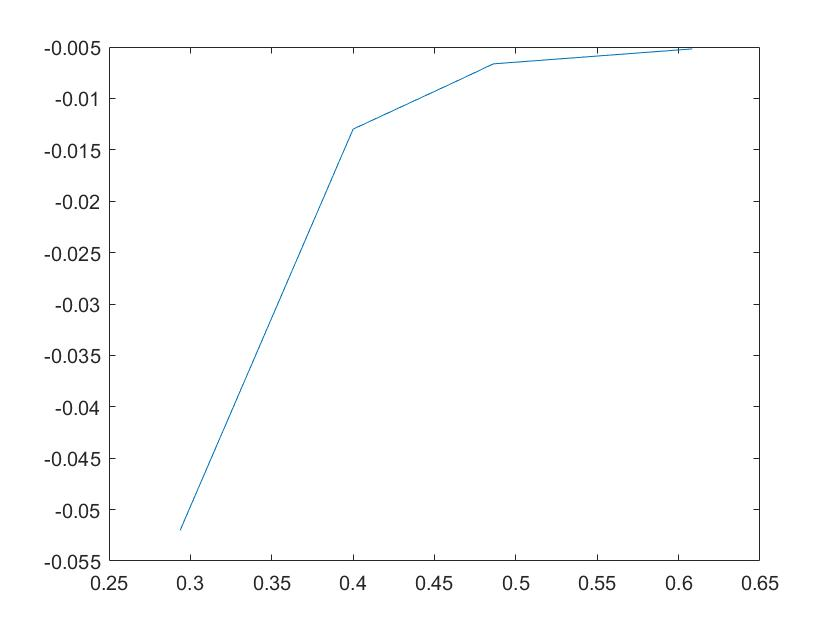
\includegraphics[height=4cm]{sd8.jpg}
		\caption{sensitivity of kd8}
	\end{subfigure}
	\caption{Sensitivity analysis of kd1-kd8}
\end{figure}
Note:The ordinate axis represents the sensitivity S, and the abscissa axis is the parameter k for which we want to evaluate the sensitivity.
\subsection{Application of the model}
Since the goal of our project is to increase the sensitivity of biosensors by introducing a complex of dCas9-RNAP and sgRNA, and one of the purposes of our model is to explore whether this complex is effective. So we assume a reasonable and large enough concentration value for this complex. We use the concentration of glyceraldehyde-3-phosphate dehydrogenase A as the assumed concentration. Glyceraldehyde 3 phosphate dehydrogenase A (gapA) is a crucial enzyme in the glycolytic pathway, and the gene encoding this enzyme is a housekeeping gene in E. coli cells with high expression levels. We find in the literature that the protein mass of gapA is 48645fg/cell, and its molecular weight is 35492 Da.\cite{Molecular \& Cellular Proteomics} The amount of abundance of Glyceraldehyde 3 phosphate dehydrogenase A protein per cell can be calculated as follows:

\begin{displaymath}
	n=\frac{m}{M}=\frac{48645*10^{-15}g}{35492g/mol}=1.37*10^{-15}mol
\end{displaymath}

As for the size of E. coli, we found relevant data from the literature, as the figure below shows.\cite{grossman1982changes}

\begin{figure}[!htbp]
	\centering
	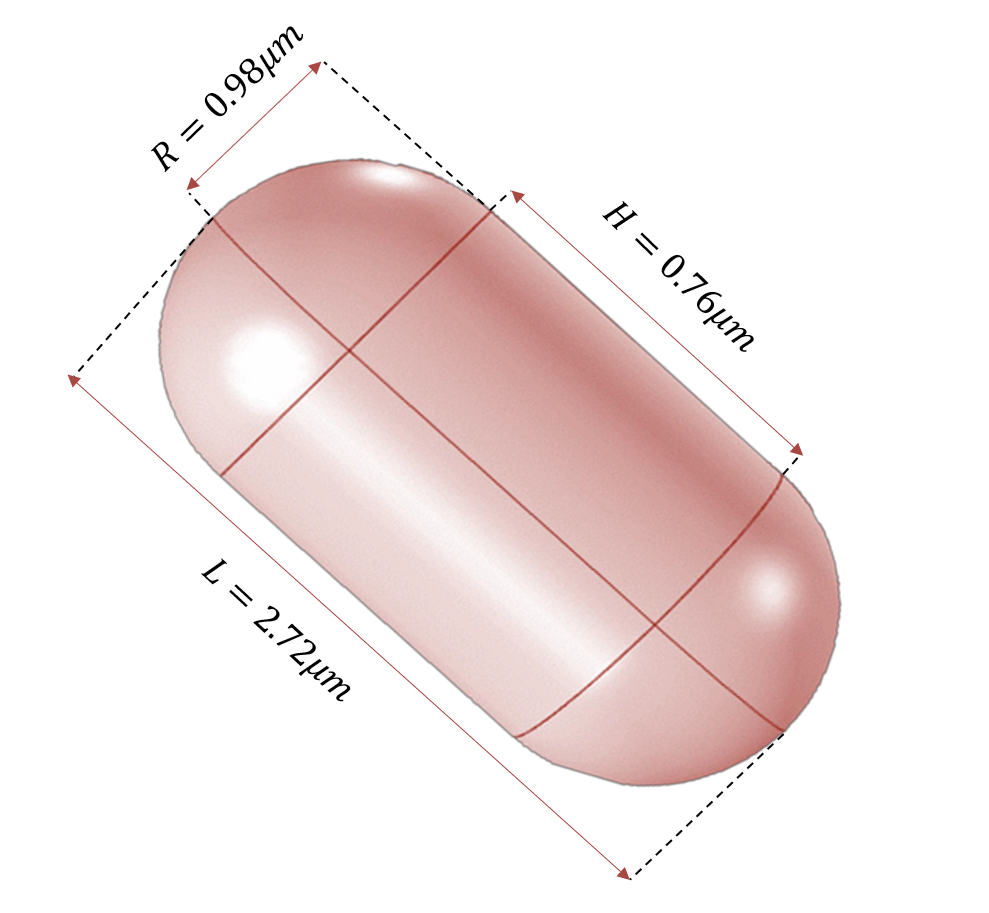
\includegraphics[width=7cm,height=7cm]{dc}
	\caption{Size of E. coli}
\end{figure}

The volume of E. coli can be calculated as follows:
\begin{displaymath}
	V_{E.coli}=\frac{4}{3} \pi R^3+\pi R^2H=\frac{4}{3} \pi (0.98\mu m)^3+\pi (0.98\mu m)^2(0.76\mu m)=6.24\mu m^3=6.24*10^{-15}L
\end{displaymath}

Then the concentration of Glyceraldehyde 3 phosphate dehydrogenase A protein in the cell can be determined:
\begin{displaymath}
	c=\frac{n}{V_{E.coli}}=\frac{1.37*10^{-15}mol}{6.24*10^{-15}L}=0.22mol/L
\end{displaymath}

With this concentration, we can get very nice results:

\begin{figure}[!htbp]
	\centering
	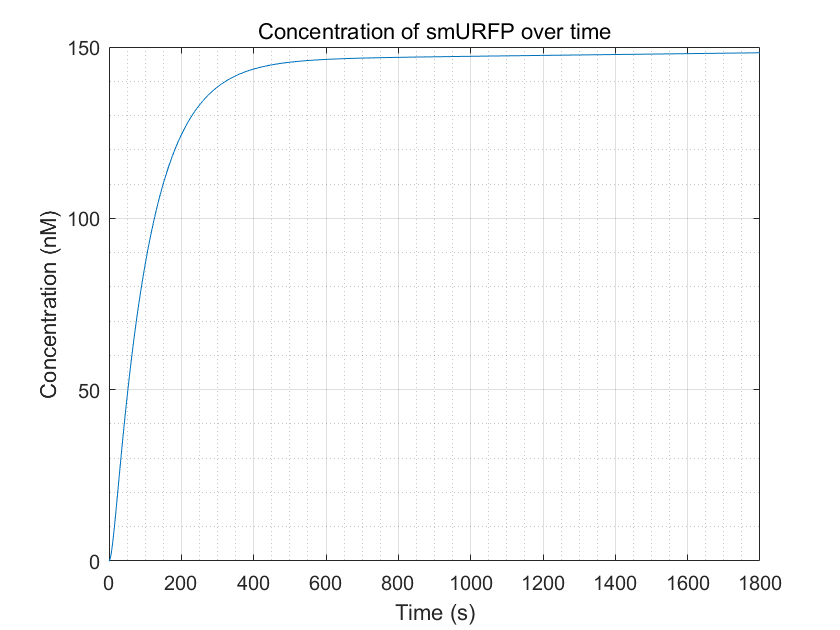
\includegraphics[width=7cm,height=7cm]{23}
	\caption{Schematic diagram of smURFP fluorescence}
\end{figure}

Compared to the diagram without introducing dCas9:

\begin{figure}[!htbp]
	\centering
	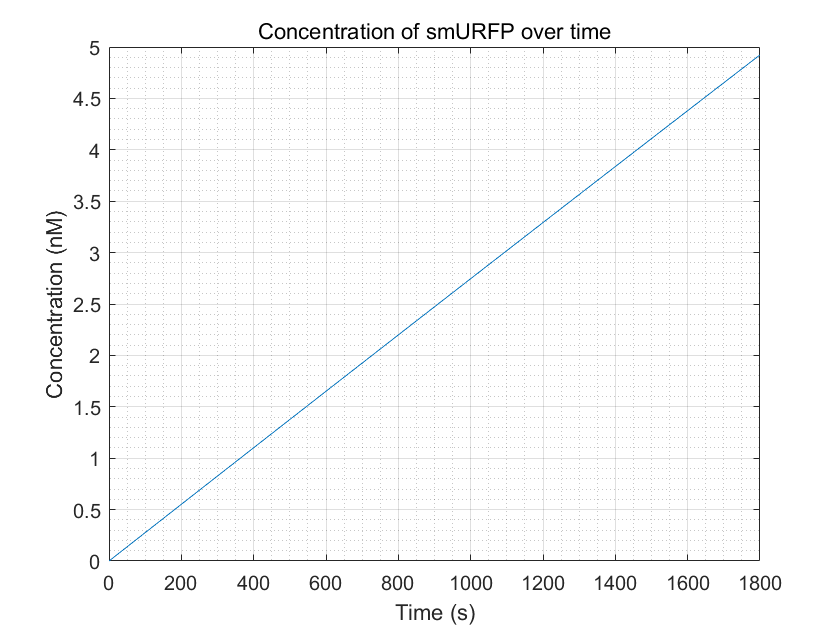
\includegraphics[width=7cm,height=7cm]{21}
	\caption{smURFP fluorescence within a reasonable time frame}
\end{figure}
\begin{figure}[!htbp]
	\centering
	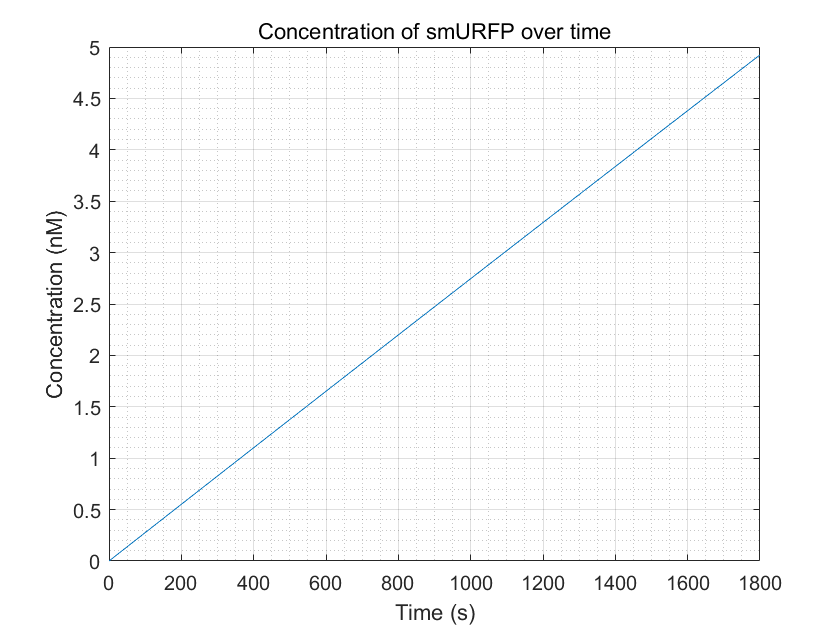
\includegraphics[width=7cm,height=7cm]{21}
	\caption{smURFP fluorescence reaches equilibrium but costs too long}
\end{figure}

From these three figures, we can conclude that dCas9-RNAP:sgRNA does have the effect of promoting transcription and increasing fluorescence intensity, thereby increasing sensitivity, as long as its concentration is sufficient. This result enhances the confidence of the experimental group, and they need to try to improve the expression of dCas9-RNAP:sgRNA in E. coli without having to doubt its role.



